Consider the tree from figure [REF]. In the figure, we have depicted/represented in each vertex last bytes of the key in hexadecimal (big endian). 

\begin{figure}[h]
	\centering
	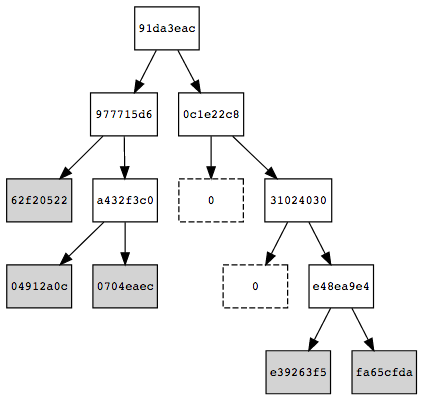
\includegraphics[scale=0.5]{images/ex-MT-5.png}
% 	http://webgraphviz.com/
%        digraph hierarchy {
%        node [fontname=Monospace,fontsize=10,shape=box]
%        "91da3eac" -> {"977715d6" "0c1e22c8"}
%        "977715d6" -> {"62f20522" "a432f3c0"}
%        "62f20522" [style=filled];
%        "a432f3c0" -> {"04912a0c" "0704eaec"}
%        "04912a0c" [style=filled];
%        "0704eaec" [style=filled];
%        "empty0" [style=dashed,label=0];
%        "0c1e22c8" -> {"empty0" "31024030"}
%        "empty1" [style=dashed,label=0];
%        "31024030" -> {"empty1" "e48ea9e4"}
%        "e48ea9e4" -> {"e39263f5" "fa65cfda"}
%        "e39263f5" [style=filled];
%        "fa65cfda" [style=filled];
%        }
\end{figure}

Now we want to store a new entry $e$ that has $H_{path}=0111111...$. First leaf we have coincides with the entry 0704eaec. So, we have to look at both paths, $H_{path}=0111110...$. So, the first different bit is bit TAL, so, we have to go down to level such and store ... in the left and ... in the right. Note that the rest of siblings are empty nodes. How the root and intermediate nodes have changed.

\begin{figure}[h]
	\centering
	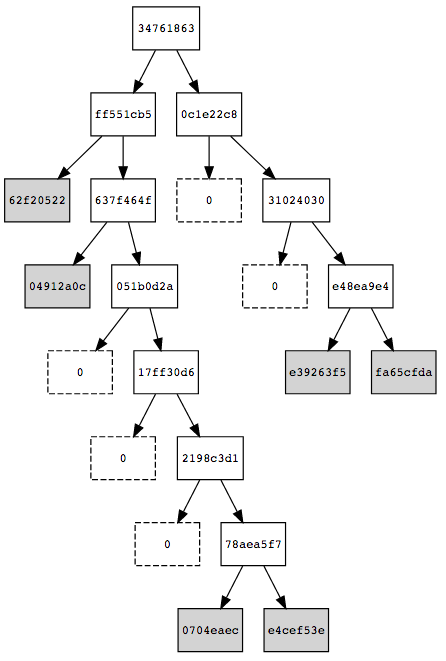
\includegraphics[scale=0.5]{images/ex-MT-6.png}
%        http://webgraphviz.com/	
%        digraph hierarchy {
%        node [fontname=Monospace,fontsize=10,shape=box]
%        "34761863" -> {"ff551cb5" "0c1e22c8"}
%        "ff551cb5" -> {"62f20522" "637f464f"}
%        "62f20522" [style=filled];
%        "637f464f" -> {"04912a0c" "051b0d2a"}
%        "04912a0c" [style=filled];
%        "empty0" [style=dashed,label=0];
%        "051b0d2a" -> {"17ff30d6" "empty0"}
%        "empty1" [style=dashed,label=0];
%        "17ff30d6" -> {"2198c3d1" "empty1"}
%        "empty2" [style=dashed,label=0];
%        "2198c3d1" -> {"empty2" "78aea5f7"}
%        "78aea5f7" -> {"0704eaec" "e4cef53e"}
%        "0704eaec" [style=filled];
%        "e4cef53e" [style=filled];
%        "empty3" [style=dashed,label=0];
%        "0c1e22c8" -> {"empty3" "31024030"}
%        "empty4" [style=dashed,label=0];
%        "31024030" -> {"empty4" "e48ea9e4"}
%        "e48ea9e4" -> {"e39263f5" "fa65cfda"}
%        "e39263f5" [style=filled];
%        "fa65cfda" [style=filled];
%        }	
\end{figure}

%\begin{center}
%\begin{tikzpicture}[auto,node distance=1.5cm] %, sibling distance=10em]
%%  level distance=20mm,
%%  text depth=.1em,
%%  text height=.8em,
%%  level 1/.style={sibling distance=10em},
%%  level 2/.style={sibling distance=20em},
%%  level 3/.style={sibling distance=20em},
%%  level 4/.style={sibling distance=10em}]
% \node [internal] (a){ } %root
%  child { node [internal]  (b) { }
%    		child {node [internal] (d) { }
%			child {node [leaf] (h) { }}
%			child {node [leaf] (i) { }}
%			}
%    		child {node [empty] (e) {asdfasdf }}
%  	}
%   child { node [internal] (c) { }
%    		child {node [empty] (f) { }}
%    		child {node [internal] (g) { }
%			child {node [internal] (j) { }
%				child{node [leaf, fill = green] (l) { } }
%				child{node [leaf] (m) { } }
%			}
%			child {node [empty] (k) { }}	
%		}
%  	};
%\end{tikzpicture}
%\end{center}

